\documentclass{beamer}
\usepackage{tcolorbox}
\usepackage{amsmath}

%\beamerdefaultoverlayspecification{<+->}
\newcommand{\data}{\mathcal{D}}

\DeclareMathOperator*{\argmin}{arg\,min}

\newcommand\Item[1][]{%
	\ifx\relax#1\relax  \item \else \item[#1] \fi
	\abovedisplayskip=0pt\abovedisplayshortskip=0pt~\vspace*{-\baselineskip}}


\usetheme{metropolis}           % Use metropolis theme


\title{Maths for ML}
\date{\today}
\author{Nipun Batra}
\institute{IIT Gandhinagar}
\begin{document}
  \maketitle
  
  
  
% \section{Linear Regression}

\begin{frame}{Contour Plot}
 $f(x,y) = x^{2} + y^{2}$\\
 Then plot $f(x,y)=K$ for varying K.
 \begin{center}
     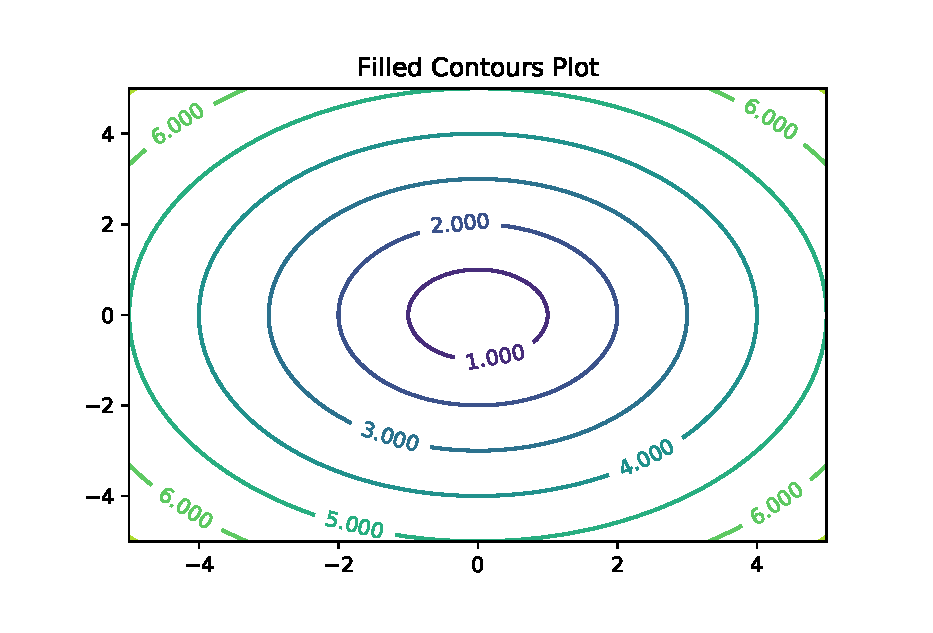
\includegraphics[totalheight=6cm]{ml-maths/contour-plot-1.eps}
 \end{center}
 
\end{frame}





\begin{frame}{Contour Plot}
    Draw the contour plot for $f(x) = x^{2}$\\
    Plot $x^{2}=K$
     \begin{center}
     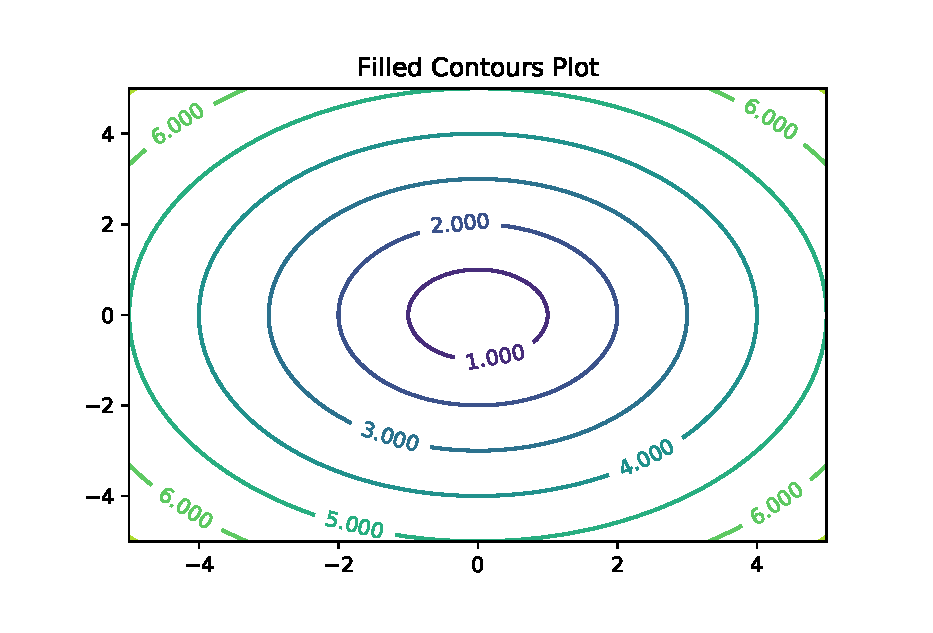
\includegraphics[totalheight=6cm]{ml-maths/contour-plot-1.eps}
 \end{center}
 
\end{frame}








\begin{frame}{Contour Plot}
    Draw the contour plot for $f(x,y) = \vert x \vert + \vert y \vert $\\
    
    Plot $\vert x \vert + \vert y \vert = K$\\
     \begin{center}
     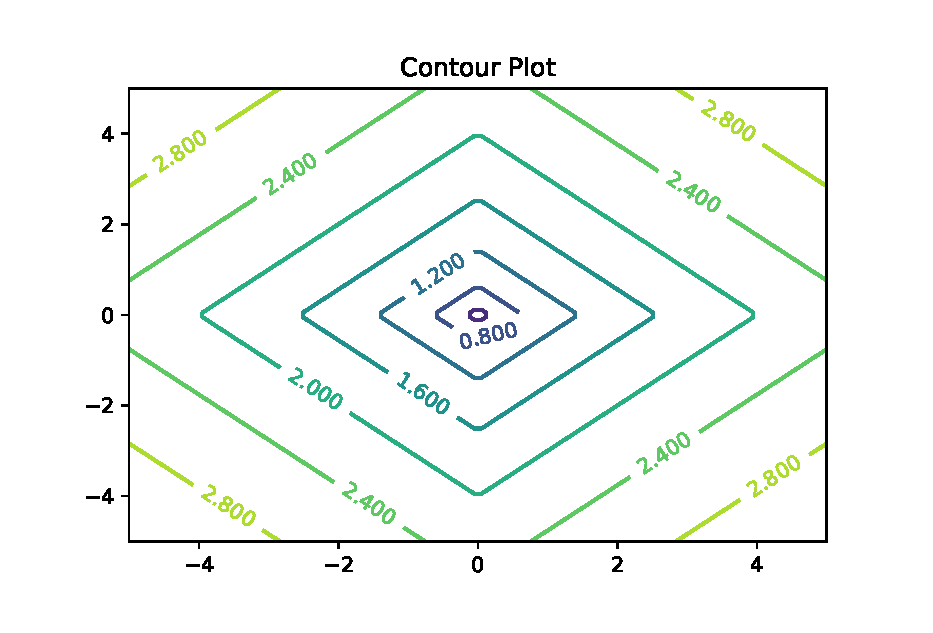
\includegraphics[totalheight=6cm]{ml-maths/contour-plot-3.eps}
 \end{center}
\end{frame}



\begin{frame}{Contour Plot}
    Draw the contour plot for $f(x,y) = x^{2}y$\\
    \begin{equation*}
        x^{2}y = K
    \end{equation*}
    
    \begin{equation*}
        y = \frac{K}{x^{2}}
    \end{equation*}
\end{frame}

\begin{frame}{Contour Plot}
    Draw the contour plot for $f(x,y) = x^{2}y$\\
    \begin{center}
     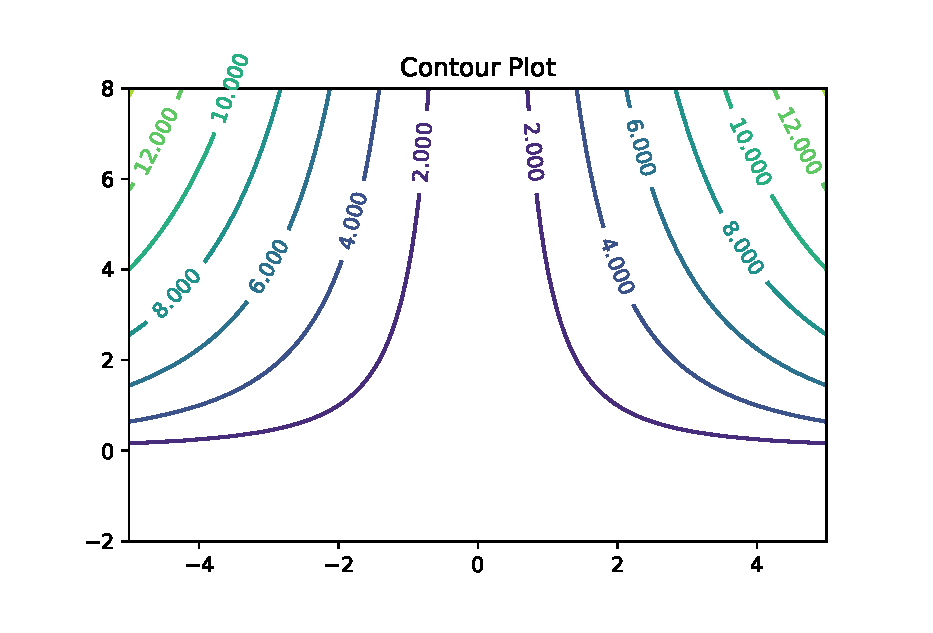
\includegraphics[totalheight=6cm]{ml-maths/contour-plot-4.eps}
 \end{center}
\end{frame}


\begin{frame}{Contour Plot}
    Draw the contour plot for $f(x,y) = xy$\\
    \begin{equation*}
        xy = K
    \end{equation*}
    
    \begin{equation*}
        y = \frac{1}{x}
    \end{equation*}
\end{frame}

\begin{frame}{Contour Plot}
    Draw the contour plot for $f(x,y) = xy$\\
        \begin{center}
     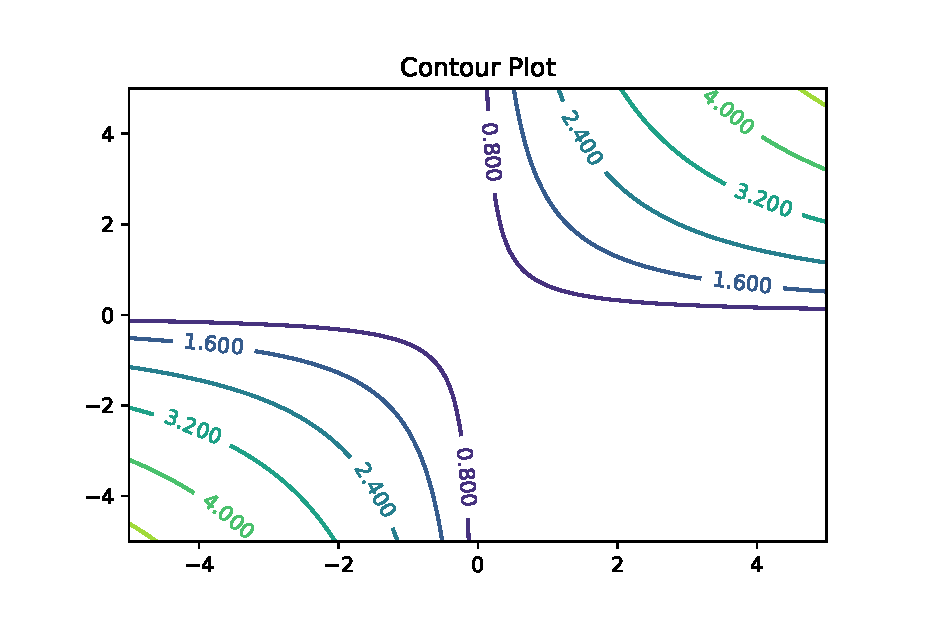
\includegraphics[totalheight=6cm]{ml-maths/contour-plot-5.eps}
 \end{center}
\end{frame}



\begin{frame}{Contours plots and gradients}
    
    
    Gradient denotes the steepest change.\\
    All points on the contour have the same $f(x,y)$\\
    
    
\end{frame}

\begin{frame}{Contours plots and gradients}
    
     \begin{center}
     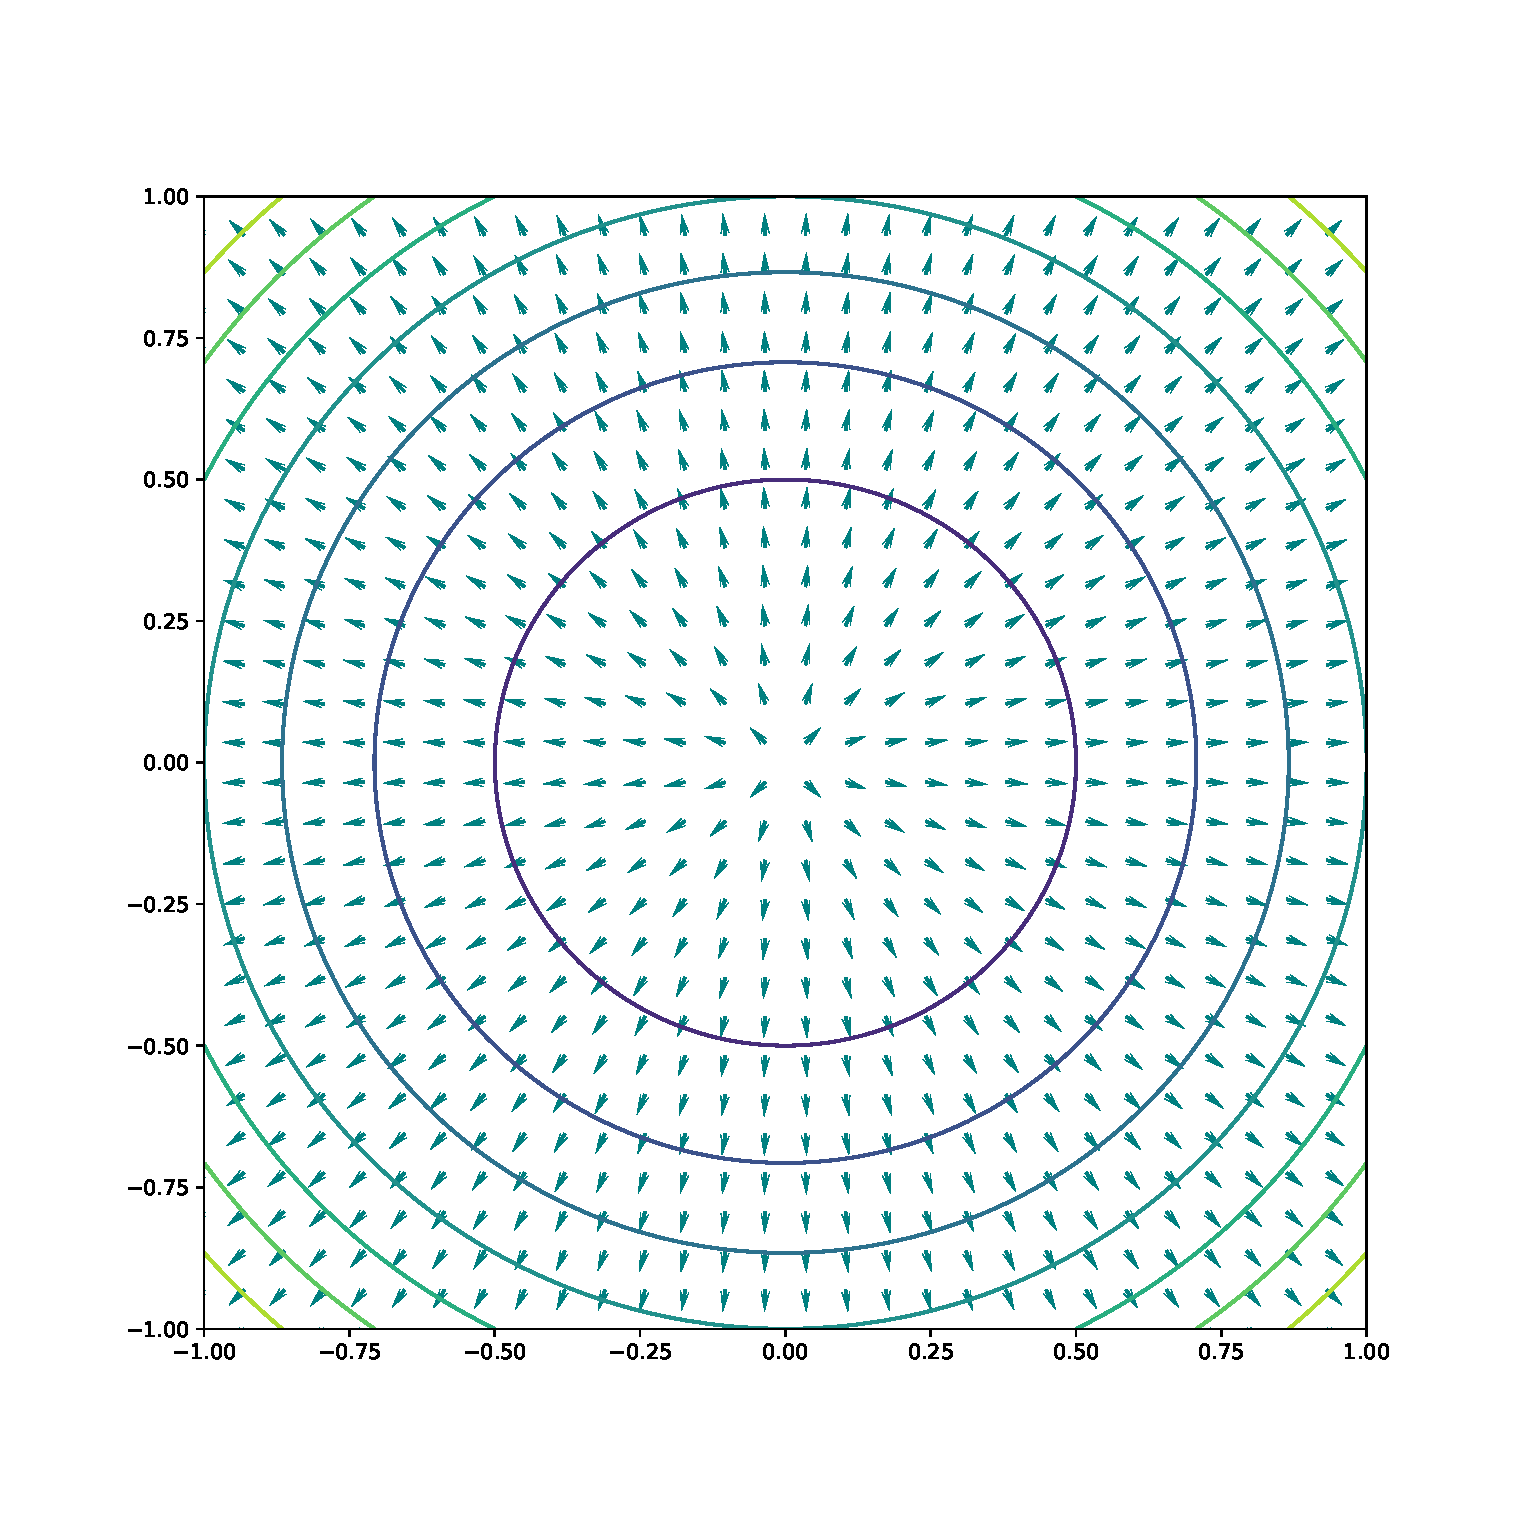
\includegraphics[totalheight=6cm]{ml-maths/gradient-field.eps}
 \end{center}
    
    
\end{frame}







\begin{frame}{Contour Plots and Gradients}
    
    Gradient denotes the direction of steepest descent.\\
    All points on the contour have the same f(x,y).\\
    Gradient denotes the direction in which there is a maximum increase in f(x,y)\\

    
    
\end{frame}



% \begin{frame}{Contour PLots and Gradients}
    
    
%     Assume f(x,y) = $x^{2}+y^{2}$.\\
    
    
%     \begin{equation*}
%         \nabla f(x,y) = \begin{bmatrix}
%             \frac{\partial }{\partial x} f(x,y)\\
%             \frac{\partial }{\partial y} f(x,y)
%         \end{bmatrix}
%     \end{equation*}
    
%     \begin{equation*}
%         \nabla f(x,y) = 
%         2
%         \begin{bmatrix}
%         x\\
%         y
%         \end{bmatrix}
%     \end{equation*}
    
% \end{frame}


\begin{frame}{Constrained Optimization}
    
    Extreme (max or min) $f(x,y) = x^{2}+y^{2}$ s.t $xy=k$\\
    
    \vspace{5em}
    More generally Extrema f(x,\dots) s.t g(x,\dots) = 0
    
\end{frame}

\begin{frame}{Constrained Optimization}
    
    $\nabla f(x,y) = \lambda g(x,y)$\\
    $\nabla f(x,y) = \begin{bmatrix}
    2x\\
    2y
    \end{bmatrix}
    = \lambda \nabla g(x,y)  = \lambda \begin{bmatrix}
    y\\
    x\\
    \end{bmatrix}$
\end{frame}

\begin{frame}{Constrained Optimization}
    
    \begin{equation}
            2x = \lambda y
    \end{equation}
    
    
    \begin{equation}
            2y = \lambda x
    \end{equation}
    
    
    \begin{equation}
            xy = \lambda k
    \end{equation}
    
    \textbf{k is a constant}
\end{frame}

\begin{frame}{Constrained optimization}
    We have three equations involving three variables. 
    On solving the above equations, we get\\
    x = y = $\sqrt{k}$\\
    $\lambda = 2$\\
\end{frame}

\begin{frame}{Constrained Optimization}
    Extrema(max or min) of $f(x,y) = x^{2} + y^{2}$ s.t $x + y = 1$\\
    
    \vspace{5em}
    More generally Extrema f(x,\dots) s.t g(x,\dots) = 0
\end{frame}

\begin{frame}{Constrained Optimization}
    $\nabla f(x,y) = \lambda g(x,y)$ \\
    \vspace{1em}
    $$
   \nabla f(x, y)=\left[\begin{array}{l}
   	{2 x} \\
   	{2 y}
   \end{array}\right] 
    \vspace{10em} 
    \nabla g(x, y)=\left[\begin{array}{l}
    	{1} \\
    	{1}
    \end{array}\right]
    $$
\end{frame}

\begin{frame}{Constrained Optimization}
    \begin{equation}
        2x=\lambda
    \end{equation}
    \begin{equation}
        2y=\lambda
    \end{equation}
    \begin{equation}
        x + y - 1 = 0
    \end{equation}
    On solving we get x = y = 0.5
\end{frame}

\begin{frame}{Constrained Optimization}

\end{frame}

\begin{frame}{Lagrangian Multiplier}
    Lagrangian $L(x,y,\lambda)$
    \begin{itemize}
        \item $\cfrac{\partial L}{\partial x} = 0$
        \item $\cfrac{\partial L}{\partial y} = 0$
        \item $\cfrac{\partial L}{\partial \lambda} = 0$
    \end{itemize}
    
\end{frame}


\begin{frame}{Lagrangian Multiplier}
    Find the extrema of $f(x,y) =x^{2}y$ s.t $g(x,y)=x^{2}+y^{2} = 1$ \\
    \vspace{1em}
    $L = x^{2}y + \lambda (x^{2} + y^{2} - 1)$\\
    \vspace{1em}
    Compute the partial derivatives
\end{frame}

\begin{frame}{Lagrangian Multiplier}
    \begin{equation}
        \cfrac{\partial L}{\partial x} = 0 \implies 2xy + \lambda(2x) = 0
    \end{equation}
    
    \begin{equation}
        \cfrac{\partial L}{\partial y} = 0 \implies x^{2} + \lambda(2y) = 0
    \end{equation}
    
    \begin{equation}
        \cfrac{\partial L}{\partial \lambda} = 0 \implies x^{2} + y^{2} - 1 = 0
    \end{equation}
\end{frame}

\begin{frame}{Case 1}
    x = 0\\
    \vspace{1em}
    f(x,y) = 0\\
    \vspace{1em}
    $y^{2} = 1 \implies y= \pm 1$\\
    \vspace{1em}
    $\lambda = 0$
\end{frame}

\begin{frame}{Case 2}
    x $\neq  \implies y = \lambda$
    \vspace{1em}
    $x^{2} = 2\lambda^{2}$ substitute the above values in Equation 9
    \vspace{1em}
    $3\lambda^{2} = 1 \implies \lambda = \pm \cfrac{1}{\sqrt{3}}$
    \vspace{1em}
    $y = \pm \cfrac{1}{\sqrt{3}}$
    \vspace{1em}
    Max of $x^{2}y = \cfrac{2}{3} \sqrt{\cfrac{1}{3}}$
\end{frame}


\begin{frame}{KKT Conditions}
    Minimize f(x)\\
    such that $h_{i} = 0 \hspace{1em} \forall i = 1 \dots m$\\
    such that $g_{i} \leq 0 \hspace{1em} \forall j = 1 \dots n$\\
    
    \begin{equation*}
        L(x,\lambda,\mu)= f(x) + \sum_{i=1}^{n}\lambda_{i}h_{i}(x) + 
        \sum_{i=1}^{m}\mu_{i}g_{i}(x) 
    \end{equation*}
    Now, if $g_{i}(x^{*})<0$, then $\mu_{i}$ can be set to zero.\\
    else  $g_{i}(x^{*})=0$\\
    Therefore $\mu_{i}g_{i}(x^{*})=0 \implies \mu_{i}>0$
\end{frame}


\begin{frame}{Lagrange Multiplier}
    Stationarity\\
    \begin{equation*}
        \nabla_{x}f(x) + \sum_{i=1}^{m} \nabla_{x}\lambda_{i}h_{i}(x)+\sum_{i=1}^{m}\nabla_{x}\mu_{i}g_{i}(x)=0
    \end{equation*}
    Equality
    \begin{equation*}
        \nabla_{x}f(\lambda) + \sum_{i=1}^{m} \nabla_{\lambda}\lambda_{i}h_{i}(x)+\sum_{i=1}^{m}\nabla_{\lambda}\mu_{i}g_{i}(x)=0
    \end{equation*}
    Inequality
    \begin{equation*}
        \mu_{i}g_{i}=0 \implies \mu_{i} \geq 0
    \end{equation*}
\end{frame}
\end{document}